\documentclass[12pt]{article}
\usepackage[margin=1in]{geometry}
\usepackage[utf8]{inputenc}
\usepackage{graphicx}
\usepackage{pdfpages}
\usepackage{hyperref}
\usepackage{setspace}
\usepackage[title]{appendix}
\graphicspath{ {./Figures/} }
\hypersetup{
	colorlinks=true,
	linkcolor=blue,
	filecolor=magenta,      
	urlcolor=cyan,
}
\urlstyle{same}
\usepackage[font={small,it}]{caption}
\usepackage{fancyvrb}
\title{Time Series Analysis \& Forecasting of Samsung Galaxy Search Trends}
\author{John D. Bulger, Craig Garzella\\
	Analytics \& Modeling
	\\Valparaiso University, Valparaiso, IN\thanks{``We have neither given or received, nor have we tolerated others' use of unauthorized aid."}}
\date{Presentation: April 30, 2019}

\begin{document}
	\maketitle
	
	\section{Introduction}
	
	Samsung, a global conglomerate, offers an enormous product line.  These include computers, appliances, wearables, and mobile devices, among many others.  Their Galaxy line, premium mobile phones, often have the highest consumer levels impact and attention.  The annual releases of the Galaxy S and Galaxy Note devices over the past several years garner a large amount of speculatory articles, leaks, and reviews.  Upon release, many service providers and retailers offer pre-order and purchase deals and bundles with these devices.
	
	\par
	
	
	Google Trends is a free service that offers an unparalleled look into Google Search activity.  Any search term can be viewed over a custom time frame, filtered by demographic region.  Famously, this service gave rise to the Google Flu Trends, where the start of flu season can be identified earlier by analyzing Googlers' symptom searches.  Similarly, this service allows for search trends to be shown not just for exact terms, but on general topics.  Results are shown as a time series, with points shown as relative search levels.
	
	\par
	
	The goal of this analysis is to develop an explanatory time series model for the search impact of the Samsung Galaxy product line.  Seasonality, as well as a general trend, are expected to be present in such data.  By creating an appropriate ARIMA model, it will then be possible to predict search impact for the next product release cycle in 2020.
	
	\section{Data}
	
	The data for this analysis consist of 76 data points spanning 2013-2019 for Google searches for the ``Samsung Galaxy" product line.\cite{data}  Each point represents a monthly search ``index" level as calculated by Google.  The data is freely available at the Google Trends site by following \href{https://trends.google.com/trends/explore?q=\%2Fm\%2F0hnbsn3\&geo=US}{this link}.  For this analysis, the data will be split into the first 64 points (for model estimation) and the remaining final 12 points (for forecast analysis).  These two subsets of the data can be seen in their entirety in Appendices A \& B.
	
	\section{Preliminary Analysis}
	
	The entire data set, plotted over time, can be seen in Figure 1.
	
\begin{figure}
		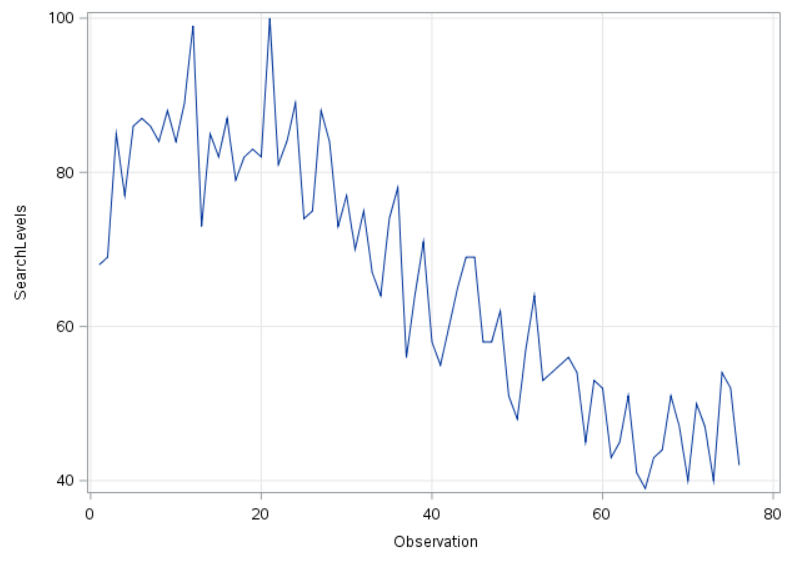
\includegraphics[scale=.7]{All_Plot.png}
		\caption{Samsung Galaxy search levels, 01/2013-04/2019}
\end{figure}

	
\paragraph{Trend}

	Upon examining the plot of the data, a clear downward trend can be seen, especially in the years 2015-2017.  This trend appears to level off both early and late in this time series.

\paragraph{Seasonality}

	This data does contain seasonality, with spikes occurring annually in March and September, as well as during the holiday season.  March and September are historically release times for the Galaxy S and Galaxy Note devices, so an increased search interest is expected around those times.  Furthermore, being a consumer-centric product, an increase in interest around the holidays is to be expected.

\paragraph{Nonstationarity}
	
	This data does not appear to be particularly nonstationary.  The standardized monthly data levels partially prevent this; additionally, the current trajectory does not appear to be heading towards either $ \infty $ or $ -\infty $.  However, upon conducting the Dickey-Fuller test prior to model specification, a difference may still need to be taken to ensure stationarity.
	

\paragraph{Outliers}

	No outliers exist in this data sample.  The search index levels are standardized by Google on a scale from 1-100; as a result, all of the data points fall within this range.  No outlier treatment is necessary prior to analysis of this data.

\newpage
\begin{thebibliography}{1}
	
		
	\bibitem{data}
	Google Trends. (2019). \textit{Samsung Galaxy: Product Line} [Data file]. Retrieved from https://trends.google.com/trends/explore?q=\%2Fm\%2F0hnbsn3\&geo=US.
	
	
	
\end{thebibliography}

\newpage
\begin{appendices}	
	\section{Modeling Data Subset}
	
	\begin{figure}[h!]
		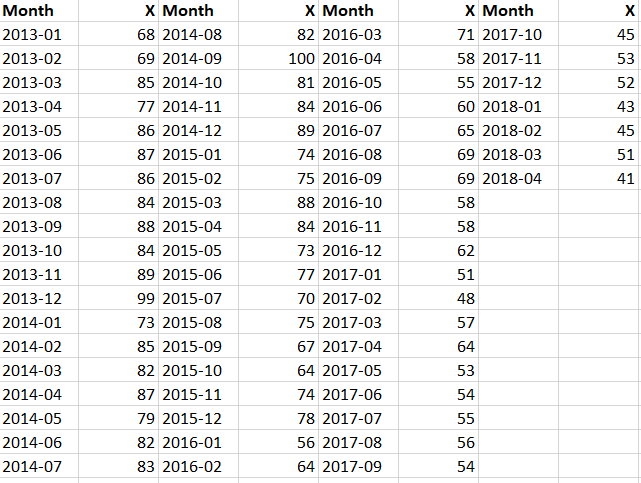
\includegraphics[scale=1.1]{Data_Table_Model.png}
	\end{figure}

\newpage

	\section{Forecasting Data Subset}

\begin{figure}[h!]
	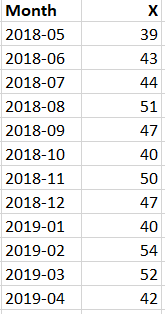
\includegraphics[scale=1.1]{Data_Table_Forecast.png}
\end{figure}

\end{appendices}




\end{document}